

\documentclass[8pt]{beamer}
\usetheme{default}
\PassOptionsToPackage{usenames,dvipsnames}{xcolor}
\usepackage{my_pres}
\usepackage{tikz}
\usepackage{empheq,accents}
\usepackage{pifont}
\usetikzlibrary{arrows}



% Created by S. Boyd and L. Vandenberghe 
% some traditional definitions that can be blamed on craig barratt
\newcommand{\BEAS}{\begin{eqnarray*}}
\newcommand{\EEAS}{\end{eqnarray*}}
\newcommand{\BEA}{\begin{eqnarray}}
\newcommand{\EEA}{\end{eqnarray}}
\newcommand{\BEQ}{\begin{equation}}
\newcommand{\EEQ}{\end{equation}}
\newcommand{\BIT}{\begin{itemize}}
\newcommand{\EIT}{\end{itemize}}

% text abbrevs
\newcommand{\eg}{{\it e.g.}}
\newcommand{\ie}{{\it i.e.}}

% std math stuff
\newcommand{\ones}{\mathbf 1}
\newcommand{\reals}{{\mbox{\bf R}}}
\newcommand{\integers}{{\mbox{\bf Z}}}
\newcommand{\complex}{{\mbox{\bf C}}}
\newcommand{\symm}{{\mbox{\bf S}}}  % symmetric matrices

% lin alg stuff
\newcommand{\Span}{\mbox{\textrm{span}}}
\newcommand{\range}{{\mathcal R}}
\newcommand{\nullspace}{{\mathcal N}}
\newcommand{\Rank}{\mathop{\bf rank}}
\newcommand{\Tr}{\mathop{\bf tr}}
\newcommand{\cond}{\mathop{\bf cond}}
\newcommand{\diag}{\mathop{\bf diag}}
\newcommand{\lambdamax}{\lambda_{\rm max}}
\newcommand{\lambdamin}{\lambda_{\rm min}}

% probability stuff
\newcommand{\Prob}{\mathop{\bf prob}}
\newcommand{\Expect}{\mathop{\bf E{}}}
\newcommand{\var}{\mathop{\bf var}} % variance
% not sure why we have \Expect and \Prob but \var ???

% convexity & optimization stuff
\newcommand{\Co}{\mathop {\bf conv}} % convex hull
\newcommand{\argmin}{\mathop{\rm argmin}}
\newcommand{\argmax}{\mathop{\rm argmax}}
\newcommand{\epi}{\mathop{\bf epi}}
%\newcommand{\hypo}{\mathop{\bf hypo}}

% sup and inf that look OK in saddle-point form!
%\newcommand{\ourinf}{\mathop{\raisebox{0ex}[0ex][.4ex]{\,inf\,}}}
%\newcommand{\oursup}{\mathop{\raisebox{0ex}[0ex][.4ex]{\,sup\,}}}
\newcommand{\ourinf}{\mathop{\,\mathrm{inf}\, {\rule[-.5ex]{0ex}{0ex}}}}
\newcommand{\oursup}{\mathop{\,\mathrm{sup}\, {\rule[-.5ex]{0ex}{0ex}}}}
%makes latex believe that inf and sup both extend .4ex below
%the baseline

\newcommand{\dist}{\mathop{\bf dist}}
\newcommand{\vol}{\mathop{\bf vol}} % volume
\newcommand{\Card}{\mathop{\bf card}} % cardinality
\newcommand{\sign}{\mathop{\bf sign}}

\newcommand{\dom}{\mathop{\bf dom}} % domain
\newcommand{\aff}{\mathop{\bf aff}} % affine hull
\newcommand{\cl}{\mathop{\bf cl}} % closure
\newcommand{\intr}{\mathop{\bf int}} % interior
\newcommand{\relint}{\mathop{\bf rel int}} % relative interior
\newcommand{\bd}{\mathop{\bf bd}} % boundary

%why do we have the following but not \nust?
\newcommand{\xst}{x^\star}
\newcommand{\lambdast}{\lambda^\star}

% defs for cones & generalized inequalities
% these seem kind of awkward; should fix some day
% rewrite them to use args?
\newcommand{\geqK}{\mathrel{\succeq_K}}
\newcommand{\gK}{\mathrel{\succ_K}}
\newcommand{\leqK}{\mathrel{\preceq_K}}
\newcommand{\lK}{\mathrel{\prec_K}}
\newcommand{\geqKst}{\mathrel{\succeq_{K^*}}}
\newcommand{\gKst}{\mathrel{\succ_{K^*}}}
\newcommand{\leqKst}{\mathrel{\preceq_{K^*}}}
\newcommand{\lKst}{\mathrel{\prec_{K^*}}}
\newcommand{\geqL}{\mathrel{\succeq_L}}
\newcommand{\gL}{\mathrel{\succ_L}}
\newcommand{\leqL}{\mathrel{\preceq_L}}
\newcommand{\lL}{\mathrel{\prec_L}}
\newcommand{\geqLst}{\mathrel{\succeq_{L^*}}}
\newcommand{\gLst}{\mathrel{\succ_{L^*}}}
\newcommand{\leqLst}{\mathrel{\preceq_{L^*}}}
\newcommand{\lLst}{\mathrel{\prec_{L^*}}}

%\newcounter{lecture}
%\newcommand{\lecturefl}[1]{   % use with foiltex landscape
%% \addtocounter{lecture}{1}
% \refstepcounter{lecture}
% \setcounter{equation}{0}
% \setcounter{page}{1}
% \renewcommand{\theequation}{\arabic{equation}}
% \renewcommand{\thepage}{\arabic{lecture}--\arabic{page}}
% \raggedright
% \parindent 0pt
% \rightfooter{\thepage}
% \leftheader{}
% \rightheader{}
% \LogoOff
% \input header 
% \begin{center}
%% {\Large \bfseries Lecture \arabic{lecture} \\*[\bigskipamount] {#1}}
%{\Large \bfseries \arabic{lecture}.  {#1}}
% \end{center}
% \MyLogo{#1}
%}

%\newcommand{\lectureflstar}[1]{   % use with foiltex landscape
% \setcounter{equation}{0}
% \setcounter{page}{1}
% \renewcommand{\theequation}{\arabic{equation}}
% \renewcommand{\thepage}{\arabic{page}}
% \raggedright
% \parindent 0pt
% \rightfooter{\thepage}
% \leftheader{}
% \rightheader{}
% \LogoOff
% \input header 
% \begin{center}
% {\Large \bfseries #1}
% \end{center}
% \MyLogo{#1}
%}
%\newcounter{oursection}
%\newcommand{\frametitle}[1]{  % for use with foiltex landscape
% \addtocounter{oursection}{1}
%% \setcounter{equation}{0}
% \foilhead[-1.0cm]{#1}
% \LogoOn
%}

\newenvironment{algdesc}%
   {\begin{list}{}{%
    \setlength{\rightmargin}{0\linewidth}%
    \setlength{\leftmargin}{.05\linewidth}}%
    \sffamily\small
    \item[]{\setlength{\parskip}{0ex}\hrulefill\par%
    \nopagebreak{}}}%
   {{\setlength{\parskip}{-1ex}\nopagebreak\par\hrulefill} \end{list}}

\newenvironment{colm}{\left[\begin{array}{c}}{\end{array}\right]}
\newenvironment{colv}{\left(\begin{array}{c}}{\end{array}\right)}




\definecolor{texthigh}{RGB}{137, 0, 255}
\definecolor{textred}{RGB}{255, 0, 94}
\definecolor{textgreen}{RGB}{89, 232, 151}
\definecolor{textlightgray}{RGB}{170,170,170}
\definecolor{bggray}{RGB}{230,230,230}
\definecolor{textgray}{RGB}{60,60,60}

\setbeamercolor{background canvas}{bg=bggray}
\setbeamercolor{normal text}{fg=textgray}

\setbeamertemplate{enumerate items}[default]
\setbeamertemplate{itemize items}{\ding{84}}

\title{Fundamental Limits of Singular Value Based \\Signal Detection from Randomly
  Compressed \\Signal-plus-Noise Matrices}
\institute[Univ. of Michigan]{Department of Electrical Engineering and Computer
  Science\\University of Michigan\\ }
\author[N. Asendorf, R.R. Nadakuditi]{Nicholas Asendorf, Ph.D. \hspace{10ex} Prof. Raj
  Nadakuditi\\ {\small{\texttt{asendorf@umich.edu} \phantom{addk}\hspace{12ex}
      \texttt{rajnrao@umich.edu}}  }}
\date{Asilomar Conference on Signals, Systems, and Computers\\[2ex] November 11, 2015}

\newcommand{\twr}{{\sf TW}_\reals}
\newcommand{\twc}{{\sf TW}_\complex}
\newcommand{\sx}{s_{x,i}}
\newcommand{\sy}{s_{y,i}}
\newcommand{\zx}{z_{x,i}}
\newcommand{\zy}{z_{y,i}}
\newcommand{\Zx}{Z_x}
\newcommand{\Zy}{Z_y}
\newcommand{\Ux}{U_x}
\newcommand{\Uy}{U_y}
\newcommand{\Vx}{V_x}
\newcommand{\Vy}{V_y}
\newcommand{\Pxy}{P_{xy}}
\newcommand{\kx}{k_x}
\newcommand{\ky}{k_y}
\newcommand{\kxhat}{\widehat{k}_x}
\newcommand{\kyhat}{\widehat{k}_y}
\newcommand{\khatcca}{\widehat{k}_{\text{cca}}}
\newcommand{\khaticca}{\widehat{k}_{\text{icca}}}
\newcommand{\Uxhat}{\widehat{U}_x}
\newcommand{\Uyhat}{\widehat{U}_y}
\newcommand{\Sigxhat}{\widehat{\Sigma}_x}
\newcommand{\Sigyhat}{\widehat{\Sigma}_y}
\newcommand{\Vxhat}{\widehat{V}_x}
\newcommand{\Vyhat}{\widehat{V}_y}
\newcommand{\Uxtil}{\widetilde{U}_x}
\newcommand{\Uytil}{\widetilde{U}_y}
\newcommand{\Vxtil}{\widetilde{V}_x}
\newcommand{\Vytil}{\widetilde{V}_y}
\newcommand{\Uxcir}{\accentset{\circ}{U}_x}
\newcommand{\Ukcir}{\accentset{\circ}{U}_{\widetilde{K}}}
\newcommand{\Uycir}{\accentset{\circ}{U}_y}
\newcommand{\Sigxcir}{\accentset{\circ}{\Sigma}_x}
\newcommand{\Sigycir}{\accentset{\circ}{\Sigma}_y}
\newcommand{\Vxcir}{\accentset{\circ}{V}_x}
\newcommand{\Vycir}{\accentset{\circ}{V}_y}
\newcommand{\kapcir}{\accentset{\circ}{\kappa}}
\newcommand{\xii}{x_i}
\newcommand{\yii}{y_i}
\newcommand{\Tx}{\Theta_x}
\newcommand{\Ty}{\Theta_y}
\newcommand{\Txhat}{\widehat{\Theta}_x}
\newcommand{\Tyhat}{\widehat{\Theta}_y}
\newcommand{\tx}{\theta^{(x)}}
\newcommand{\ty}{\theta^{(y)}}
\newcommand{\Kxy}{K_{xy}}
\newcommand{\Kxytil}{\widetilde{K}_{xy}}
\newcommand{\Uktil}{U_{\widetilde{K}}}
\newcommand{\Vktil}{V_{\widetilde{K}}}
\newcommand{\Uktilhat}{\widehat{U}_{\widetilde{K}}}
\newcommand{\Vktilhat}{\widehat{V}_{\widetilde{K}}}
\newcommand{\kxy}{k^{xy}}
\newcommand{\defeq}{=:}
\newcommand{\Rxx}{R_{xx}}
\newcommand{\Ryy}{R_{yy}}
\newcommand{\Rxy}{R_{xy}}
\newcommand{\Rxxhat}{\widehat{R}_{xx}}
\newcommand{\Ryyhat}{\widehat{R}_{yy}}
\newcommand{\Rxyhat}{\widehat{R}_{xy}}
\newcommand{\wx}{w_x}
\newcommand{\wy}{w_y}
\newcommand{\wxt}{\widetilde{w}_x}
\newcommand{\wyt}{\widetilde{w}_y}
\newcommand{\wxicca}{\widehat{w}_x^{\text{icca}}}
\newcommand{\wyicca}{\widehat{w}_y^{\text{icca}}}
\newcommand{\wxticca}{\widetilde{w}_x^{\text{icca}}}
\newcommand{\wyticca}{\widetilde{w}_y^{\text{icca}}}
\newcommand{\wxhaticca}{\widehat{w}_x}
\newcommand{\wyhaticca}{\widehat{w}_y}
\newcommand{\Ccca}{C_{\text{cca}}}
\newcommand{\Cccahat}{\widehat{C}_{\text{cca}}}
\newcommand{\Ciccahat}{\widehat{C}_{\text{icca}}}
\newcommand{\Ciccat}{\widetilde{C}_{\text{icca}}}
\newcommand{\rank}{\text{rank}}
\newcommand{\taucca}{\tau_{\text{cca}}^\alpha}
\newcommand{\tauicca}{\tau_{\text{icca}}^\alpha}
\newcommand{\simiid}{\overset{\text{i.i.d.}}{\sim}}
\newcommand{\rhocca}{\rho_\text{cca}}
\newcommand{\rhohatcca}{\widehat{\rho}_\text{cca}}
\newcommand{\rhohaticca}{\widehat{\rho}_\text{icca}}
\newcommand{\rhoeff}{k_{\text{eff}}^{xy}}
\newcommand{\Cmcca}{C_{\text{mcca}}}
\newcommand{\Ucir}{\accentset{\circ}{U}}
\newcommand{\Vcir}{\accentset{\circ}{V}}
\newcommand{\Cmccatil}{\widetilde{C}_{\text{mcca}}}

\newcommand{\iccap}{ICCA\texttt{+} }
\newcommand{\iccaps}{ICCA\texttt{+}}
\newcommand{\Sigxtil}{\widetilde{\Sigma}_x}
\newcommand{\Sigytil}{\widetilde{\Sigma}_y}

\newcommand{\Cmccahat}{\widehat{C}_{\text{mcca}}}
\newcommand{\Cimccahat}{\widehat{C}_{\text{imcca}}}

%\newcommand{\kapcir}{\accentset{\circ}{\kappa}}
%\newcommand{\simiid}{\overset{\text{i.i.d.}}{\sim}}
%\newcommand{\twc}{{\sf TW}_\complex}

%\newcommand{\Uxcir}{\accentset{\circ}{U}_x}
%\newcommand{\Uycir}{\accentset{\circ}{U}_y}
%\newcommand{\Vxcir}{\accentset{\circ}{V}_x}
%\newcommand{\Vycir}{\accentset{\circ}{V}_y}

\begin{document}

%--- the titlepage frame -------------------------%
\begin{frame}[plain]
  \titlepage
  \addtocounter{framenumber}{-1}
\end{frame}

\begin{frame}{Data Model}

  \begin{center}
    \textbf{Signal-plus-noise Matrix}\\
    \fcolorbox{black}[HTML]{F1F1F1}{\parbox{0.5\textwidth}{
        \be
        \widetilde{X}_n= \sum_{i=1}^r\theta_i u_iv_i^T + X_n.
        \ee    
      }}
  \end{center}

  \textbf{Parameters}
  \begin{itemize}
  \item $u_i\in\complex^{n\times 1}$, $u_i^Hu_j = \delta_{i=j}$
  \item $v_i\in\complex^{N\times 1}$, $v_i^Hv_j = \delta_{i=j}$
  \item $\theta_i>0$
  \item $X_n\in\complex^{n\times N}$ random matrix with singular values
    $\sigma_1,\dots,\sigma_{\min(n,N)}$ 
  \item Empirical singular value distribution:
  \end{itemize}

  \be
  \mu_{X_n} = \frac{1}{\min(n,N)}\sum_{i=1}^{\min(n,N)}\delta_{\sigma_i}.
  \ee
\end{frame}

\begin{frame}{Signal Detection and Random Projections}

  \begin{center}
    \textbf{Goal}\\[1ex]
    \fcolorbox{black}[HTML]{F1F1F1}{\parbox{0.7\textwidth}{
        \centering
        Detect the presence of the $r$ signals
      }}
  \end{center}

  \vspace{2ex}

  \textbf{Standard Operating Procedure}
  \begin{itemize}
  \item Take SVD of $\widetilde{X}_n$ to get $\widehat{\sigma}_i$
  \item Compare singular values to a threshold to determine significance
  \item The corresponding singular vectors, $\widehat{u}_i$, estimate signals
  \end{itemize}

\vspace{2ex}

  \textbf{Challenges in High Dimensions}
  \begin{itemize}
  \item As $n,N\to\infty$, computing the SVD of $\widetilde{X}_n$ becomes prohibitive
  \end{itemize}

\vspace{2ex}

  \textbf{Idea}
  \begin{itemize}
  \item Project $\widetilde{X}_n$ to a lower dimensional space, $Y_n=P_n^H\widetilde{X}_n$
  \item $P_n\in\complex^{n\times m}$
  \item Take SVD of $Y_n$ to detect signals
  \end{itemize}

\end{frame}

\begin{frame}{Paper Goals}

  \begin{center}
    \textbf{Goals}\\
    \fcolorbox{black}[HTML]{F1F1F1}{\parbox{0.9\textwidth}{
        \begin{itemize}
        \item Quantify how $m,n,N,\theta$ affect the behavior of the singular values of
          $Y_n$
        \item Uncover fundamental signal detection limits 
        \item Compare the performance of Gaussian and unitary projection
          matrices 
        \end{itemize}
      }}
  \end{center}

  \vspace{2ex}

    \begin{columns}
      \begin{column}{0.5\textwidth}
        \begin{center}
        \textbf{Gaussian Projection Matrix}
        \end{center}
        \begin{itemize}
        \item $P_n$ has i.i.d. $\mathcal{CN}(0,1)$ entries
        \item Gaussian-like matrix, $P_n=G_n$
          \be
          G_{ij} = \begin{cases} 1 & \text{w.p. } 1/2\\ -1 & \text{w.p. } 1/2\end{cases}
          \ee
        \end{itemize}
      \end{column}
      \begin{column}{0.5\textwidth}
        \begin{center}
        \textbf{Unitary Projection Matrix}
        \end{center}
        \begin{itemize}
        \item $P_n=Q_n$ s.t. $Q_n^HQ_n = I_m$
        \item Discrete Fourier matrix, $Q_n=F$
          \be
          F_{kj} = \frac{1}{\sqrt{n}}\exp\left\{\frac{-2\pi i (k-1)(j-1)}{n}\right\}
          \ee
        \end{itemize}
      \end{column}
    \end{columns}


\end{frame}

\begin{frame}{Main Theoretical Results}

\begin{Th}[Almost sure limit of singular values of $Y_n$]
The largest $r$ singular values of  $Y_n$ exhibit the
following behavior as $n,m,N\to\infty$ with $n/N\to c_1$ and $m/n\to c_2$. 
For each fixed $1\leq i\leq r$, $\sigma_i\left(Y_n\right)$ solves
\be
\sigma_i^2\varphi_F(\sigma_i)\varphi_H(\sigma_i) = \frac{1}{\theta_i^2},
\ee
where
\be\ba
&\varphi_{F}(\sigma_i)\convas-\E{xm_{\mu_{RS|R}}\left(\sigma_i^2,x\right)}_{\mu_R}\\
&\varphi_{H}(\sigma_i)\convas-\frac{n}{N}m_{M_3}(\sigma_i^2) - \frac{1}{\sigma_i^2}\frac{n-N}{N}
\ea\ee
where 
\begin{itemize}
\item $m_{\mu_M}$ is the Stieltjes transform of a matrix $M$ defined as
$m_{\mu_{M}}(z)=\int\frac{1}{x-z}\mu_{M}(x)$ 
\item $\mu_R$ is the limiting eigenvalue density of either $G_nG_n^H$ or $Q_nQ_n^H$
\item $\mu_S$ is the limiting eigenvalue density of $X_nX_n^H$
\item $m_{\mu_{RS|S}}$ is the
Stieltjes transform of the limiting conditional density
\item $m_{\mu_{M_3}}$ is the
Stieltjes transform of $G_nG_n^HX_nX_n^H$ or $Q_nQ_n^HX_nX_n^H$. 
\end{itemize}
\end{Th}


\end{frame}

\begin{frame}{Corollaries}

\begin{Corr}[Fundamental detection limit]
Define the critical SNR threshold as
\be
\theta_{\text{crit}} = \frac{1}{b\sqrt{\varphi_F(b)\varphi_H(b)}}.
\ee
When $\theta_i<\theta_{\text{crit}}$, then 
\be
\sigma_i\convas b,
\ee
where $b$ is the almost sure limit of the largest singular value of $P_n^HX_n$.
\end{Corr}


\begin{Corr}[Closed form solution for unitary $P$]
When $Y_n$ is a generated using a unitary matrix $Q_n$, we have that
for each fixed $1\leq i\leq r$,
\be
\sigma_i \convas \begin{cases} \sqrt{\frac{c_1}{\theta_i^2}+c_2\theta_i^2+1+c_1c_2} & \text{if }
  \theta_i\geq\left(\frac{c_1}{c_2}\right)^{1/4}\\ \sqrt{c_1c_2} +1 & \text{if }
    \theta_i<\left(\frac{c_1}{c_2}\right)^{1/4} \end{cases}.
\ee
\end{Corr}

\end{frame}

\begin{frame}{Empirical Results - Singular Value Prediction}

\begin{itemize}
\item Parameters: $r=1$, $n=1000$, $N=1220$ and $m=100$, $500$ trials
\end{itemize}

\begin{figure}
  \begin{center}
    \subfigure[Gaussian $G$]{
      \label{fig:chpt7:gauss_pred}
      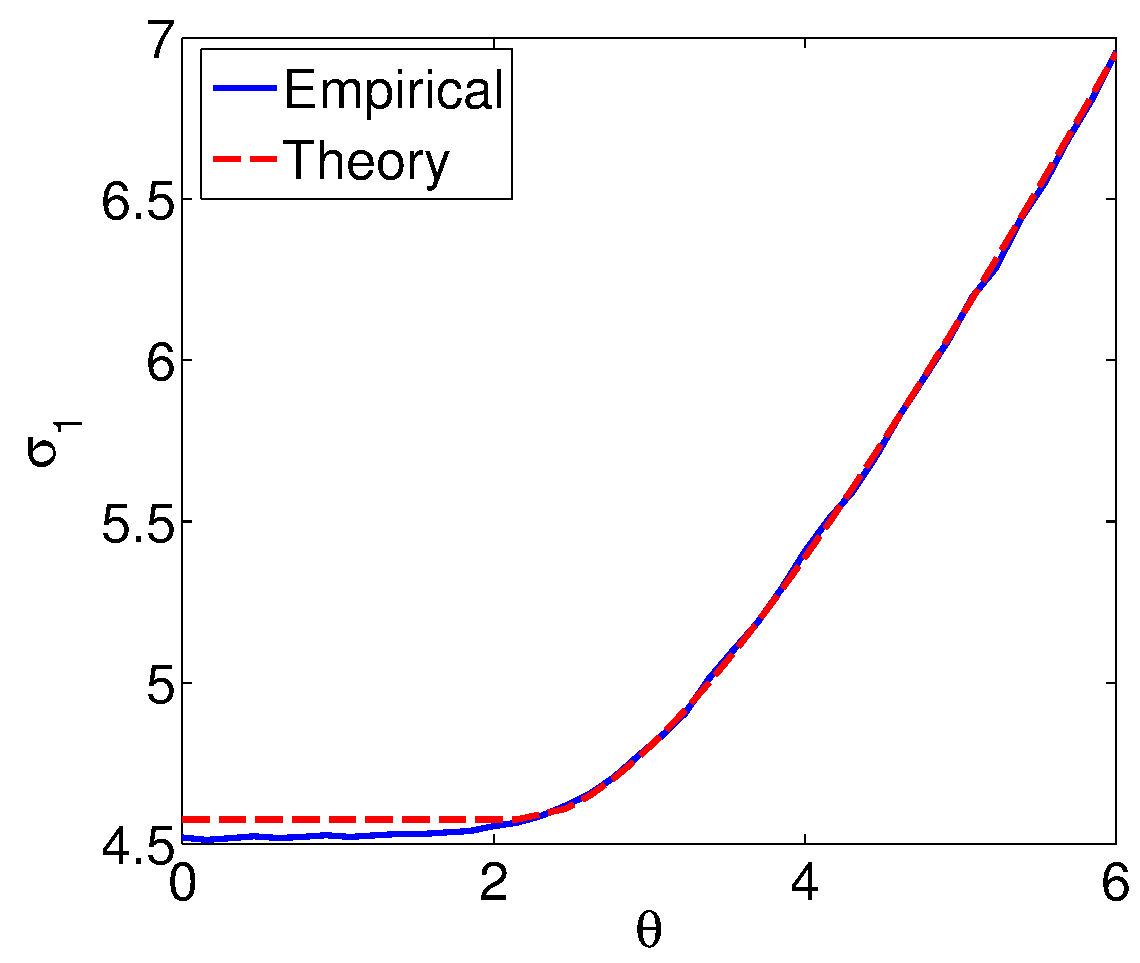
\includegraphics[width=0.36\textwidth]{chpt7_svd_proj/figs/gauss_sv_pred.pdf}
    }
    \subfigure[Gaussian-like $G$]{
      \label{fig:chpt7:gauss_like_pred}
      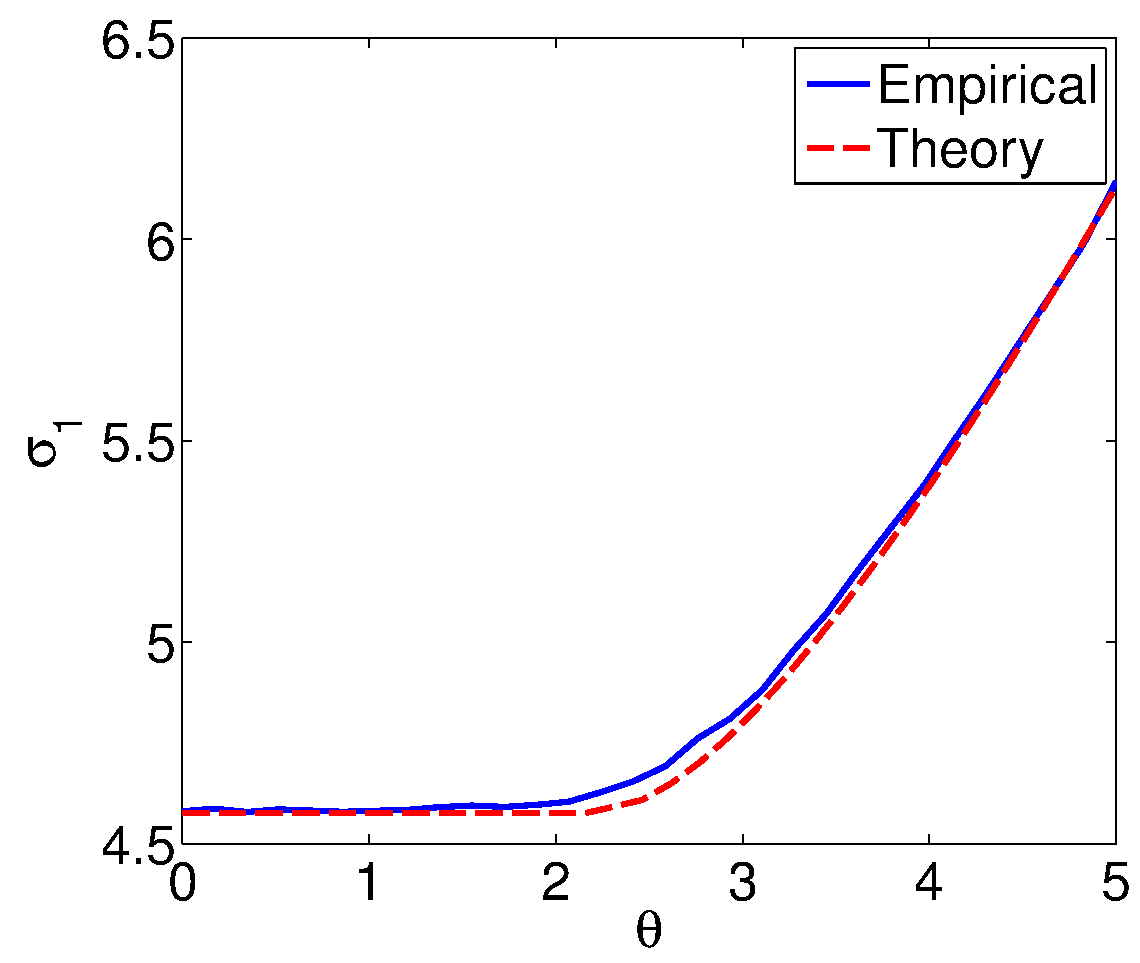
\includegraphics[width=0.36\textwidth]{chpt7_svd_proj/figs/gauss_sweep.pdf}
    }
    \subfigure[Unitary $Q$]{
      \label{fig:chpt7:ortho_pred}
      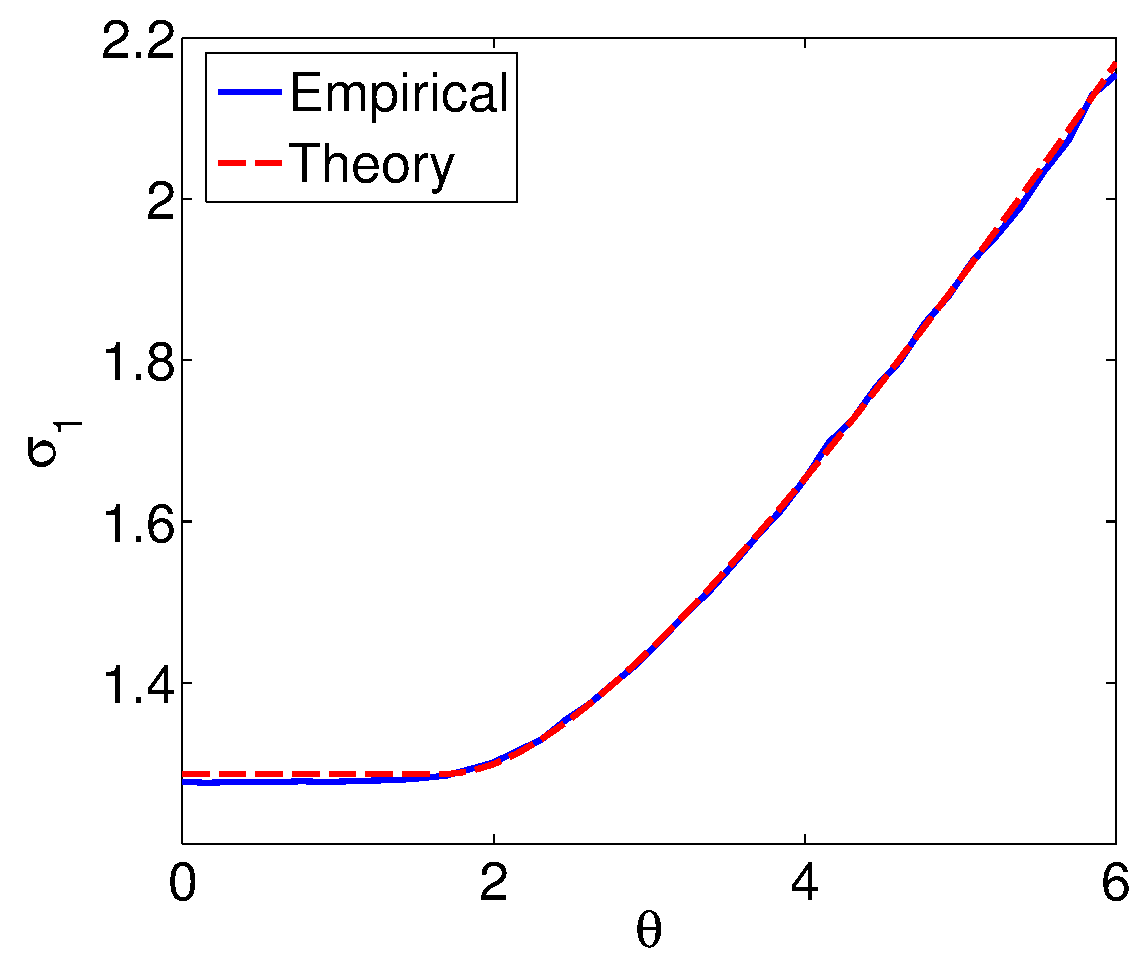
\includegraphics[width=0.36\textwidth]{chpt7_svd_proj/figs/unitary_sv_pred.pdf}
    }
    \subfigure[Fourier $Q$]{
      \label{fig:chpt7:fourier_pred}
      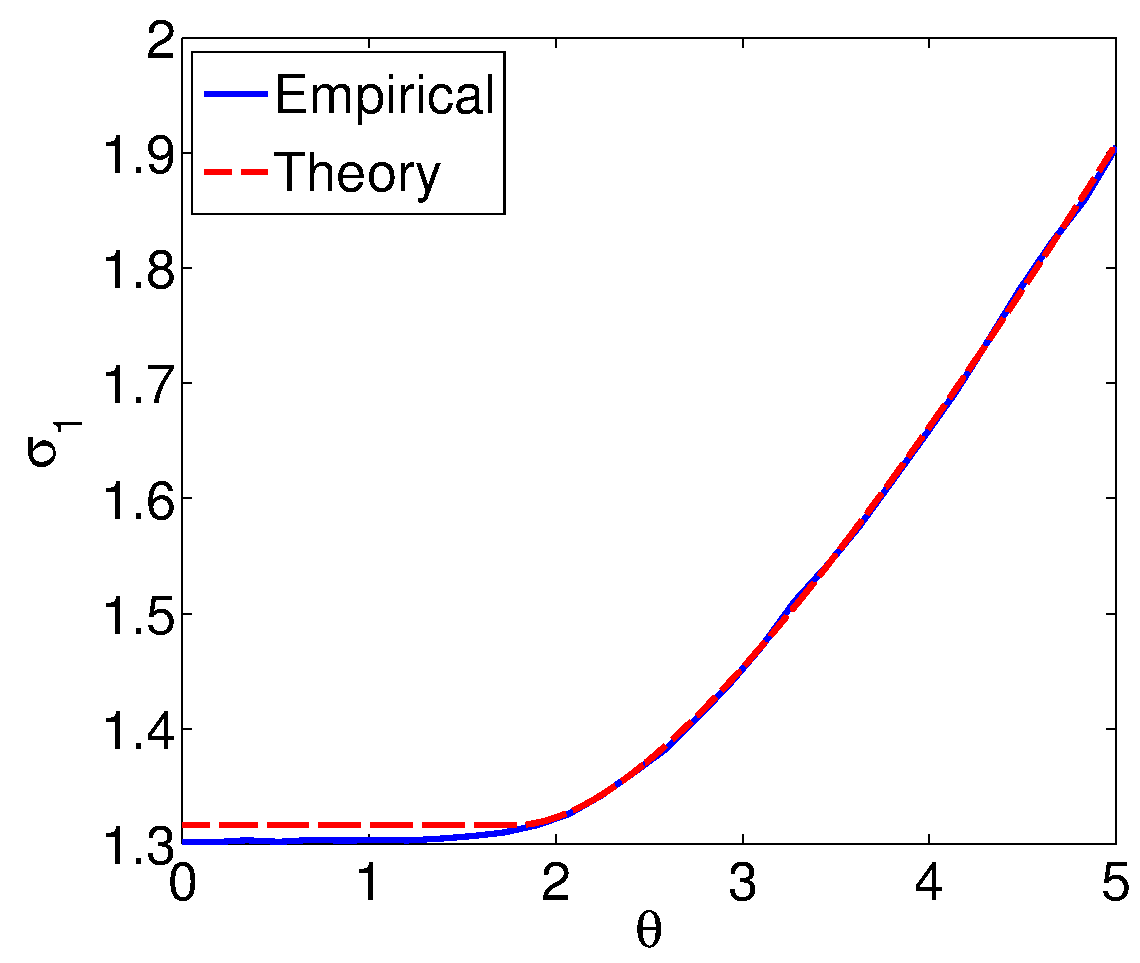
\includegraphics[width=0.36\textwidth]{chpt7_svd_proj/figs/fourier_sweep.pdf}
    }
  \end{center}
\end{figure}

\end{frame}

\begin{frame}{Empirical Results - Phase Transition Prediction}
\begin{itemize}
\item KS Statistic:  $r=1$, $n=1000$, $500$ trials
\end{itemize}

\vspace{-1ex}

\begin{figure}
\begin{center}
  \subfigure[Gaussian $m=100$]{
    \label{fig:chpt7:gauss1}
    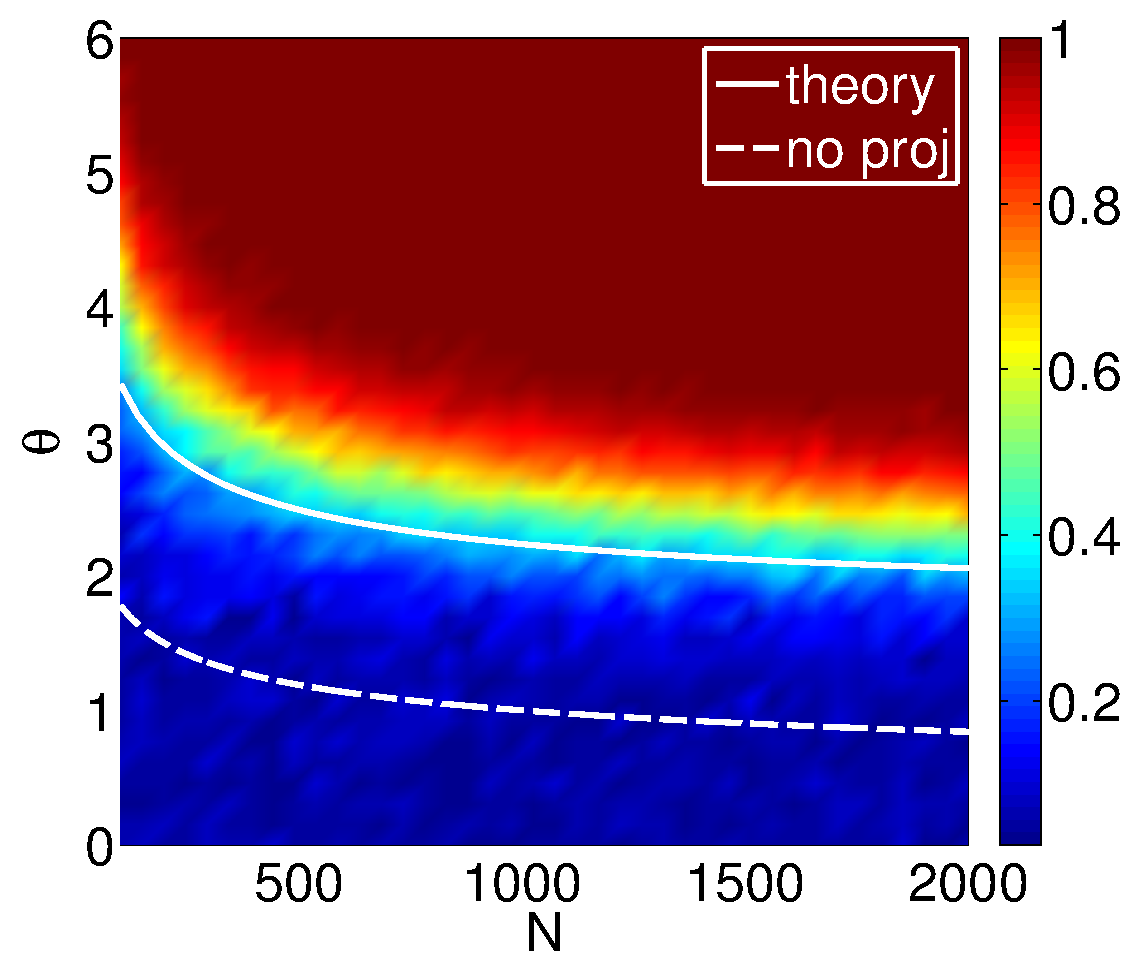
\includegraphics[width=0.36\textwidth]{chpt7_svd_proj/figs/ks11.pdf}
  }
  \subfigure[Gaussian $N=1000$]{
    \label{fig:chpt7:gauss2}
    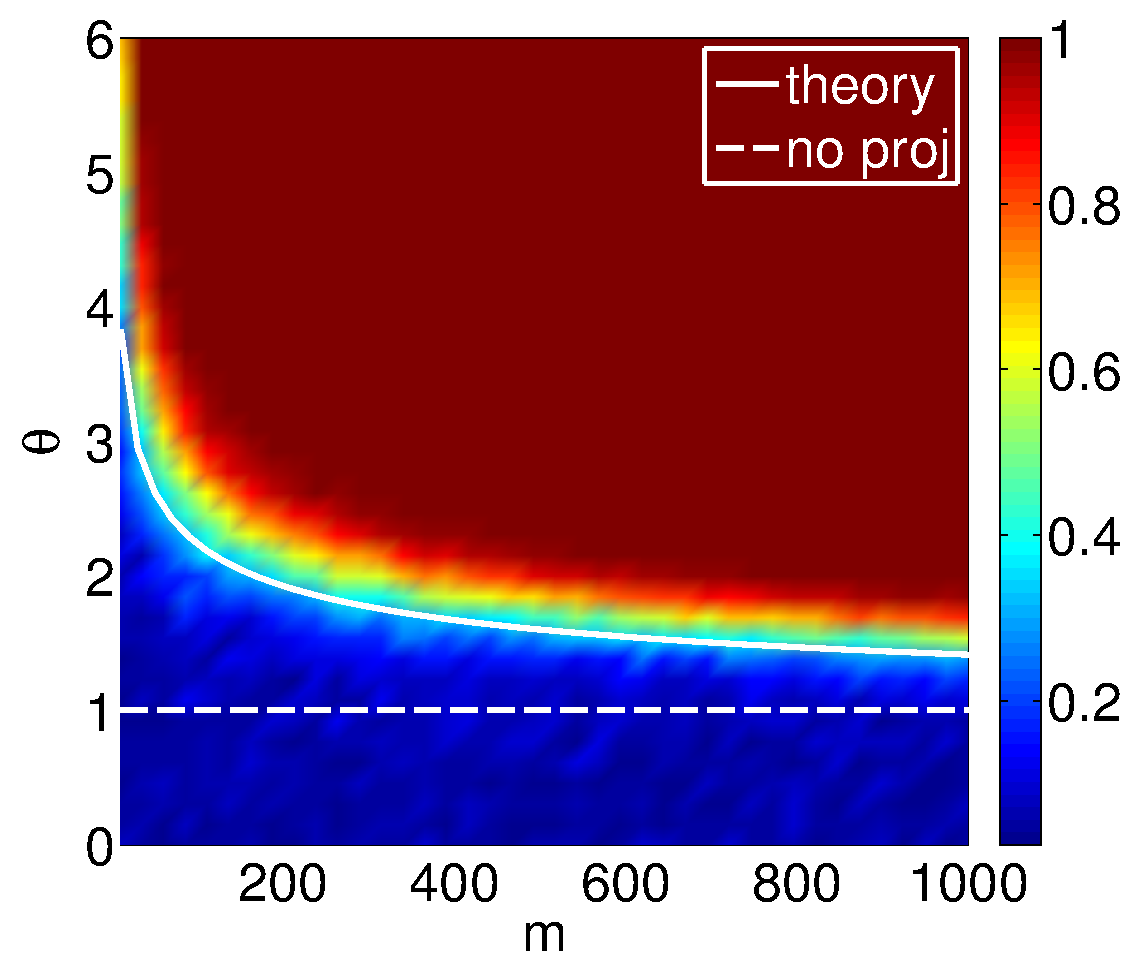
\includegraphics[width=0.36\textwidth]{chpt7_svd_proj/figs/ks21.pdf}
  }
  \subfigure[Unitary $m=100$]{
    \label{fig:chpt7:ortho1}
    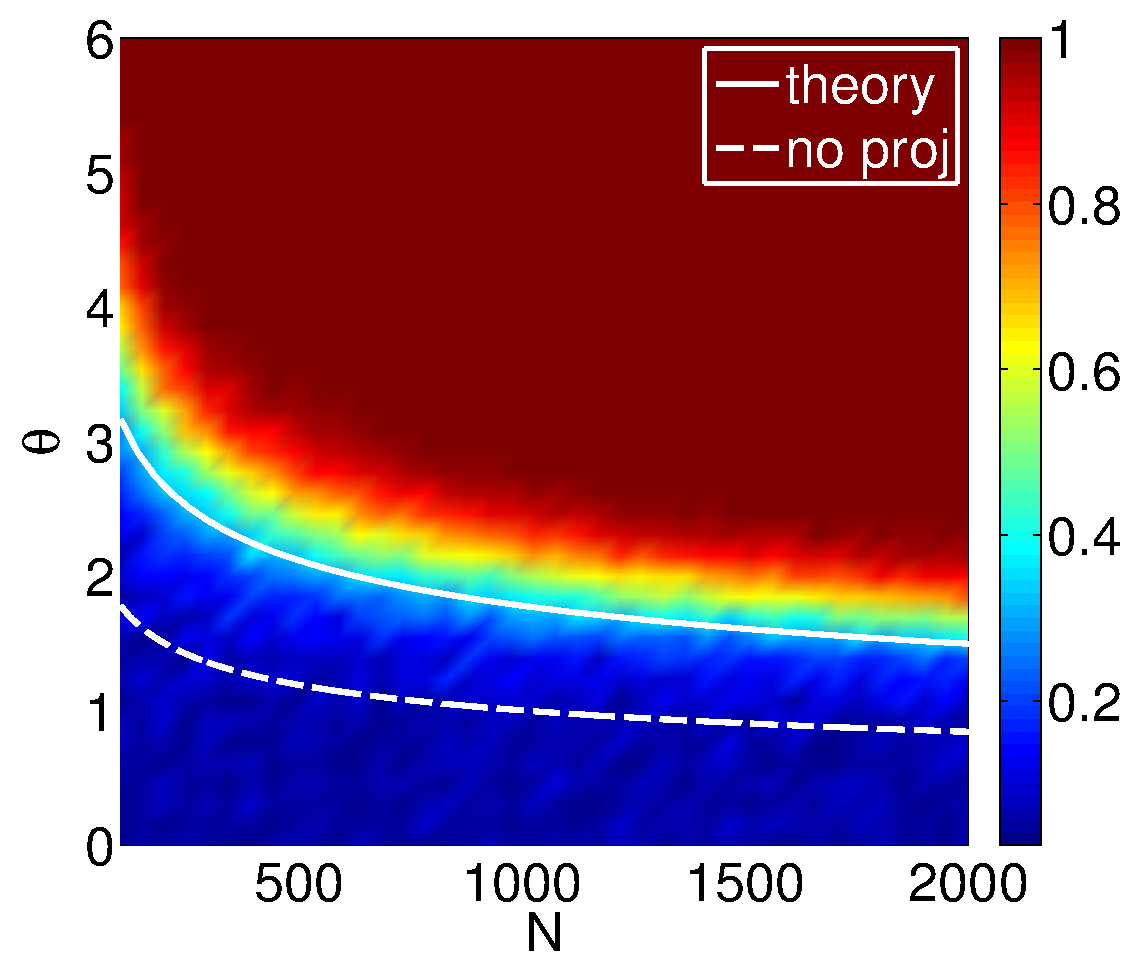
\includegraphics[width=0.36\textwidth]{chpt7_svd_proj/figs/ks12.pdf}
  }
  \subfigure[Unitary $N=1000$]{
    \label{fig:chpt7:ortho2}
    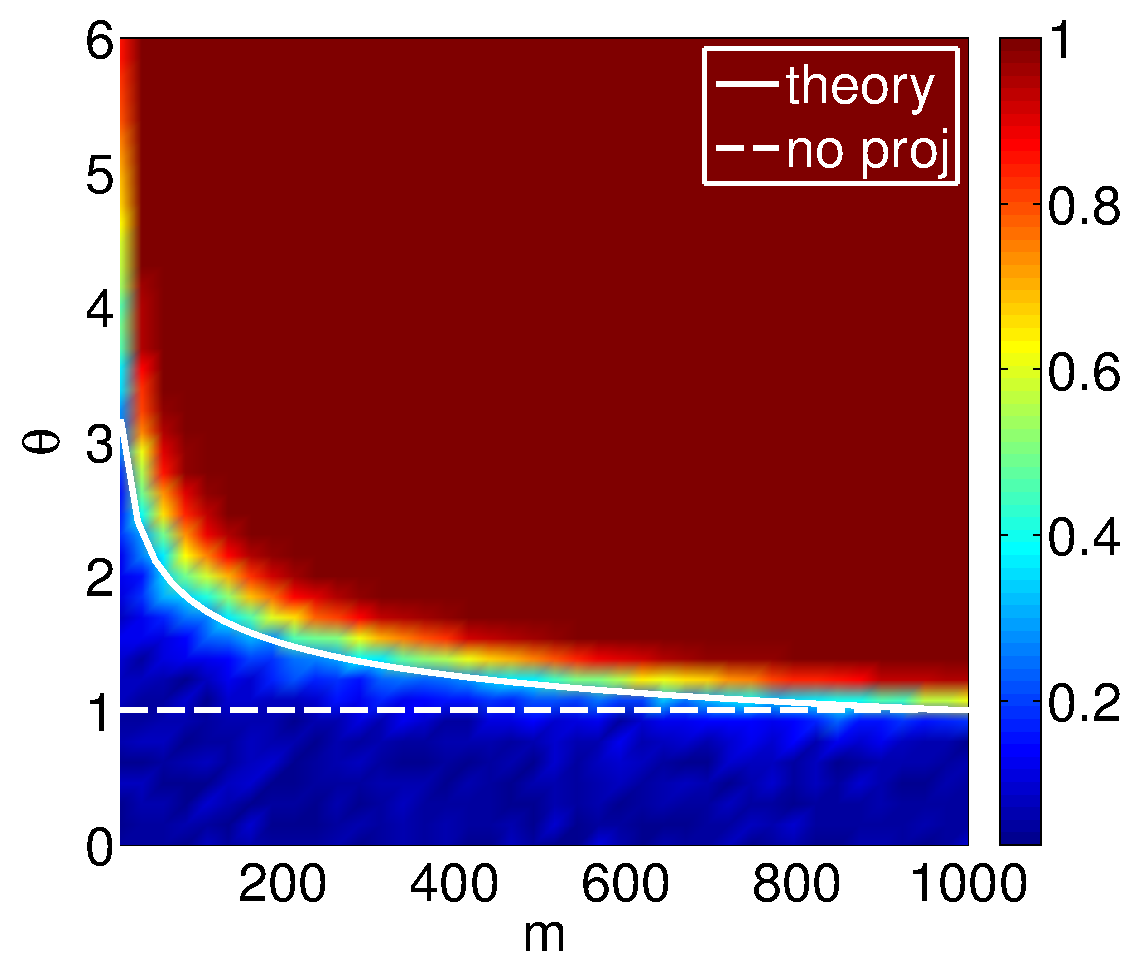
\includegraphics[width=0.36\textwidth]{chpt7_svd_proj/figs/ks22.pdf}
  }
\end{center}
\end{figure}
\end{frame}

\begin{frame}{Discussion and Conclusion}

  \textbf{Takeaways}
  \begin{itemize}
  \item Accurately predict top singular values
  \item Accurately predict detection limit
  \item Unitary projection outperforms Gaussian projection
  \item Theory allows practitioners to set system parameters to achieve desired
    performance 
  \item No closed form for Gaussian - relies on numerical techniques
  \end{itemize}
  
  \vspace{2ex}

  \textbf{Generating projection matrices}
  \begin{itemize}
  \item Easy - Gaussian, Gaussian-like (i.i.d. entries)    
  \item Hard - Unitary 
  \item Easy - Fourier
  \end{itemize}

\end{frame}

\end{document}
